\documentclass{article}

\PassOptionsToPackage{numbers, sort&compress}{natbib}
\usepackage[main,final]{neurips_2026}

\usepackage[utf8]{inputenc}
\usepackage[T1]{fontenc}
\usepackage{url}
\usepackage{booktabs}
\usepackage{amsfonts}
\usepackage{amsmath}
\usepackage{nicefrac}
\usepackage{microtype}
\usepackage{xcolor}
\usepackage{graphicx}
\usepackage{multirow}
\usepackage{algorithm}
\usepackage{algpseudocode}
\usepackage{float}
\usepackage{wrapfig}
\setlength{\intextsep}{8pt plus 2pt minus 2pt}
\usepackage{tikz}
\usetikzlibrary{arrows.meta,positioning,fit,calc,backgrounds}

\setcitestyle{citesep={,}}
\makeatletter\def\NAT@def@citea{\def\@citea{\NAT@separator}}\makeatother
\definecolor{cblue}{HTML}{1F4E79}
\definecolor{corange}{HTML}{E8833A}
\definecolor{cgreen}{HTML}{4E9A63}
\definecolor{cgrey}{HTML}{BFBFBF}
\definecolor{cviolet}{HTML}{5B3C99}
\definecolor{cred}{HTML}{C0392B}
\usepackage{courier}
\usepackage{hyperref}
\hypersetup{colorlinks=true,linkcolor=blue!55!black,citecolor=blue!55!black,urlcolor=blue!55!black}

\title{Entity-Token World Models and Differentiable Predictive Control for Building-Agnostic HVAC Control}

\author{%
  Lorenzo Giannuzzo$^{1,2}$ \quad Daniele Salvatore Schiera$^{1,2}$ \\[4pt]
  $^{1}$Department of Energy ``Galileo Ferraris'', Politecnico di Torino, 10129 Turin, Italy \\
  $^{2}$Energy Center Lab, Politecnico di Torino, 10138 Turin, Italy \\
  {\small\texttt{lorenzo.giannuzzo@polito.it}, \texttt{daniele.schiera@polito.it}}
}

\raggedbottom
\begin{document}

\maketitle

\begin{abstract}
A single controller for the Heating, Ventilation and Air Conditioning (HVAC) systems of unseen buildings has to cope with different numbers of zones and air handlers, thermal properties and climates. This work addresses the Smart Buildings Challenge by representing every zone, air handler and hot-water system as a token of the same transformer architecture, used for both a world model of the building and the policy, and by training the policy with Differentiable Predictive Control (DPC), that is, by backpropagating the competition reward through closed-loop rollouts of 12 to 48 hours inside world models refined in on-policy rounds. On the 30 official scenarios over 14 days, the score of the Proportional-Integral-Derivative (PID) baseline falls from 0.0591 to 0.0103, mostly through a lower discomfort, and an earlier policy reaches 0.013 on the Kaggle public leaderboard. The analysis shows that the remaining loss is concentrated in the subarctic climate, that the most accurate world models differ less than the training seeds, and that a search with the true simulator still recovers about 30\% of the loss in a cold and a mild scenario.
\end{abstract}

\section{Introduction}

Heating, Ventilation and Air Conditioning (HVAC) systems are still mostly operated by rule-based logic tuned by hand for each building \cite{drgona2020mpc,wang2020rl}, since Model Predictive Control (MPC) and reinforcement learning, despite large savings, require a model or a training process specific to every building \cite{pinto2022transfer}. The Smart Buildings Challenge \cite{goldfeder2026smart}, hosted on Kaggle and built on the Smart Buildings Control Suite simulator \cite{goldfeder2024smart}, makes this obstacle explicit by asking for one policy that controls buildings never seen during development, scored by a reward that combines occupant comfort, energy cost and carbon emissions.

The approach presented here describes the building as a set of entities (zones, air handlers, the hot-water system and a global token), processed by the same transformer architecture in a world model and in the policy, so that both apply to any building, and trains the policy, neither by trial and error nor by imitation, by Differentiable Predictive Control (DPC) \cite{drgona2022dpc}, maximizing the competition reward rebuilt from the world-model predictions through closed-loop rollouts, as outlined in Figure~\ref{fig:architecture}. The main contributions of this work are the following:
\begin{itemize}
  \item an entity-token world model with long thermal memory, refined in on-policy rounds, with a closed-loop temperature error of 0.79 K after 24 hours on held-out buildings;
  \item a DPC scheme with rollouts of 12 to 24 hours, a command filter inside them and two alternated world models, which reaches 0.0103 on the 30 official scenarios, against 0.0591 for the Proportional-Integral-Derivative (PID) baseline;
  \item an analysis of where the gains come from, by reward term, climate and control behavior, of the calibration of the world models and of the spread between training seeds, together with an oracle bound on the remaining headroom.
\end{itemize}

\begin{figure}[H]
\centering
\resizebox{0.86\linewidth}{!}{%
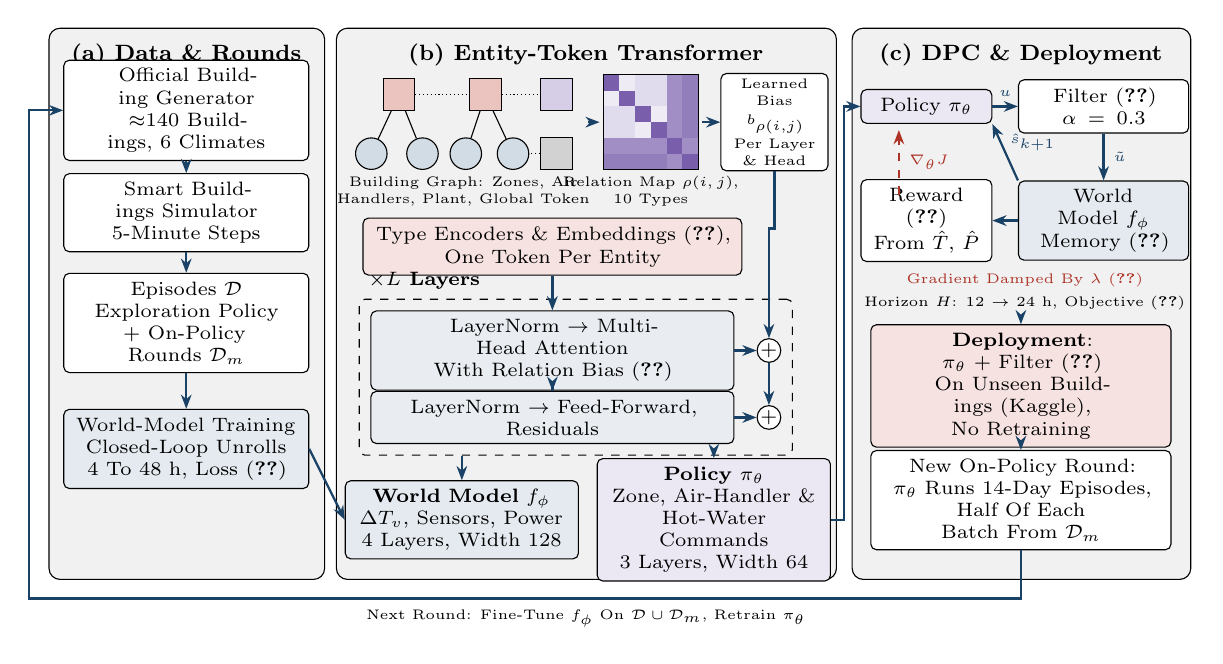
\begin{tikzpicture}[
  font=\scriptsize,
  box/.style={draw, rounded corners=2pt, align=center, inner sep=3pt, fill=white},
  arr/.style={-{Stealth[length=1.8mm]}, thick, cblue!85!black},
  grad/.style={-{Stealth[length=1.8mm]}, thick, dashed, cred!90!black},
  panel/.style={draw=black, rounded corners=4pt, fill=cgrey!22},
  zn/.style={circle, draw, fill=cblue!20, inner sep=0pt, minimum size=4mm},
  an/.style={rectangle, draw, fill=cred!30, inner sep=0pt, minimum size=4mm},
  hn/.style={rectangle, draw, fill=cviolet!25, inner sep=0pt, minimum size=4mm},
  gn/.style={rectangle, draw, fill=cgrey!70, inner sep=0pt, minimum size=4mm}]
% ---------- panels
\begin{scope}[on background layer]
\node[panel, minimum width=3.5cm, minimum height=7.0cm, anchor=north west] (PA) at (0,0) {};
\node[panel, minimum width=6.35cm, minimum height=7.0cm, anchor=north west] (PB) at (3.65,0) {};
\node[panel, minimum width=4.3cm, minimum height=7.0cm, anchor=north west] (PC) at (10.2,0) {};
\end{scope}
\node[anchor=north, font=\footnotesize\bfseries] at (1.75,-0.08) {(a) Data \& Rounds};
\node[anchor=north, font=\footnotesize\bfseries] at (6.825,-0.08) {(b) Entity-Token Transformer};
\node[anchor=north, font=\footnotesize\bfseries] at (12.35,-0.08) {(c) DPC \& Deployment};
% ---------- panel A
\node[box, text width=2.9cm] (gen) at (1.75,-1.05) {Official Building Generator\\ $\approx$140 Buildings, 6 Climates};
\node[box, text width=2.9cm] (sim) at (1.75,-2.35) {Smart Buildings Simulator\\ 5-Minute Steps};
\node[box, text width=2.9cm] (dat) at (1.75,-3.75) {Episodes $\mathcal{D}$\\ Exploration Policy\\ + On-Policy Rounds $\mathcal{D}_m$};
\node[box, text width=2.9cm, fill=cblue!12] (wmt) at (1.75,-5.35) {World-Model Training\\ Closed-Loop Unrolls\\ 4 To 48 h, Loss (\ref{eq:wmloss})};
\draw[arr] (gen) -- (sim);
\draw[arr] (sim) -- (dat);
\draw[arr] (dat) -- (wmt);
% ---------- panel B: building graph
\node[an] (a1) at (4.45,-0.85) {};
\node[an] (a2) at (5.55,-0.85) {};
\node[zn] (z1) at (4.1,-1.6) {}; \node[zn] (z2) at (4.75,-1.6) {};
\node[zn] (z3) at (5.3,-1.6) {}; \node[zn] (z4) at (5.9,-1.6) {};
\node[hn] (h) at (6.45,-0.85) {}; \node[gn] (g) at (6.45,-1.6) {};
\draw (a1)--(z1) (a1)--(z2) (a2)--(z3) (a2)--(z4);
\draw[densely dotted] (a1)--(a2)--(h) (g)--(z4);
\node[align=center, font=\tiny] at (5.27,-2.08) {Building Graph: Zones, Air\\ Handlers, Plant, Global Token};
% relation matrix
\begin{scope}[shift={(7.05,-0.6)}]
\foreach \i in {0,...,5} \foreach \j in {0,...,5} {
  \pgfmathtruncatemacro{\r}{ifthenelse(\i==\j,9,ifthenelse(\i<4 && \j<4, ifthenelse((\i<2 && \j<2) || (\i>1 && \j>1),0,1), ifthenelse(\j==4 || \i==4, 6, 7)))}
  \pgfmathsetmacro{\c}{10+8*\r}
  \fill[cviolet!\c!white] (\j*0.2,-\i*0.2) rectangle ++(0.2,-0.2);
}
\draw (0,0) rectangle (1.2,-1.2);
\end{scope}
\node[align=center, font=\tiny] at (7.65,-2.08) {Relation Map $\rho(i,j)$,\\ 10 Types};
\node[box, text width=1.22cm, font=\tiny, inner sep=2pt] (bias) at (9.22,-1.2) {Learned Bias\\[1pt] $b_{\rho(i,j)}$\\[1pt] Per Layer \& Head};
\draw[arr] (6.85,-1.2) -- (7.0,-1.2);
\draw[arr] (8.3,-1.2) -- (bias.west);
% layer stack
\node[box, text width=4.6cm, fill=cred!14] (enc) at (6.4,-2.78) {Type Encoders \& Embeddings (\ref{eq:tokens}),\\ One Token Per Entity};
\node[box, text width=4.4cm, fill=cblue!10] (att) at (6.4,-4.1) {LayerNorm $\rightarrow$ Multi-Head Attention\\ With Relation Bias (\ref{eq:attention})};
\node[box, text width=4.4cm, fill=cblue!10] (ffn) at (6.4,-4.95) {LayerNorm $\rightarrow$ Feed-Forward,\\ Residuals};
\node[draw, circle, inner sep=0pt, minimum size=3mm, fill=white] (p1) at (9.15,-4.1) {$+$};
\node[draw, circle, inner sep=0pt, minimum size=3mm, fill=white] (p2) at (9.15,-4.95) {$+$};
\begin{scope}[on background layer]
\node[draw, dashed, rounded corners=2pt, fit=(att)(ffn)(p1)(p2), inner sep=4pt] (blk) {};
\end{scope}
\node[anchor=south west, font=\scriptsize\bfseries] at (blk.north west) {$\times L$ Layers};
\draw[arr] (enc.south) -- (att.north);
\draw[arr] (att) -- (p1);
\draw[arr] (ffn) -- (p2);
\draw[arr] (p1) -- (p2);
\draw[arr] (att.south) -- (ffn.north);
\draw[arr] (bias.south) -- (9.22,-2.55) -| (p1.north);
% heads
\node[box, text width=2.75cm, fill=cblue!12] (wmh) at (5.25,-6.25) {\textbf{World Model} $f_\phi$\\ $\Delta T_v$, Sensors, Power\\ 4 Layers, Width 128};
\node[box, text width=2.75cm, fill=cviolet!12] (pih) at (8.45,-6.25) {\textbf{Policy} $\pi_\theta$\\ Zone, Air-Handler \&\\ Hot-Water Commands\\ 3 Layers, Width 64};
\draw[arr] (blk.south -| wmh) -- (wmh);
\draw[arr] (blk.south -| pih) -- (pih);
% ---------- panel C: DPC loop
\node[box, text width=1.45cm, fill=cviolet!12] (pi) at (11.15,-1.0) {Policy $\pi_\theta$};
\node[box, text width=1.95cm] (flt) at (13.4,-1.0) {Filter (\ref{eq:filter})\\ $\alpha = 0.3$};
\node[box, text width=1.95cm, fill=cblue!12] (wm) at (13.4,-2.45) {World Model $f_\phi$\\ Memory (\ref{eq:memory})};
\node[box, text width=1.45cm] (rew) at (11.15,-2.45) {Reward (\ref{eq:dpc})\\ From $\hat{T}$, $\hat{P}$};
\draw[arr] (pi) -- node[above, font=\tiny] {$u$} (flt);
\draw[arr] (flt) -- node[right, font=\tiny] {$\tilde{u}$} (wm);
\draw[arr] (wm) -- (rew);
\draw[arr] (wm.north west) -- node[above right, font=\tiny, pos=0.45, inner sep=1pt] {$\hat{s}_{k+1}$} (pi.south east);
\draw[grad] (10.8,-2.12) -- node[right, font=\tiny, text=cred!90!black] {$\nabla_\theta J$} (10.8,-1.3);
\node[font=\tiny, align=center, text=cred!90!black] at (12.4,-3.2) {Gradient Damped By $\lambda$ (\ref{eq:damp})};
\node[font=\tiny, align=center] at (12.4,-3.5) {Horizon $H$: 12 $\rightarrow$ 24 h, Objective (\ref{eq:dpc})};
\node[box, text width=3.6cm, fill=cred!14] (dep) at (12.35,-4.55) {\textbf{Deployment}: $\pi_\theta$ + Filter (\ref{eq:filter})\\ On Unseen Buildings (Kaggle),\\ No Retraining};
\node[box, text width=3.6cm] (onp) at (12.35,-6.0) {New On-Policy Round:\\ $\pi_\theta$ Runs 14-Day Episodes,\\ Half Of Each Batch From $\mathcal{D}_m$};
\draw[arr] (12.35,-3.7) -- (dep.north);
\draw[arr] (dep) -- (onp);
% ---------- cross-panel arrows
\draw[arr] (wmt.east) -- (wmh.west);
\draw[arr] (pih.east) -- (10.1,-6.25) |- (pi.west);
\draw[arr] (onp.south) -- (12.35,-7.25) -- (-0.25,-7.25) |- (gen.west);
\node[font=\tiny, anchor=north] at (6.825,-7.27) {Next Round: Fine-Tune $f_\phi$ On $\mathcal{D} \cup \mathcal{D}_m$, Retrain $\pi_\theta$};
\end{tikzpicture}}
\caption{Overview of the method: (a) data collection on generated buildings and on-policy rounds; (b) entity-token transformer shared by the world model and the policy (same structure, separate weights), with Graphormer-style attention biases given by the relation between two entities; (c) DPC training of the policy through the world model and deployment on unseen buildings.}
\label{fig:architecture}
\end{figure}

\section{Related Works}

Unlike the detailed individual test cases of the Building Optimization Testing (BOPTEST) framework \cite{blum2021boptest}, the Smart Buildings Challenge evaluates a single policy on buildings generated at scale. MPC is the reference for advanced building control \cite{drgona2020mpc}, but requires a model identified for every building. Deep reinforcement learning has been applied to HVAC control since \cite{wei2017drl}, with sample efficiency, safety and transfer to new buildings as its main obstacles \cite{wang2020rl,pinto2022transfer}.

Differentiable MPC \cite{amos2018diffmpc} embeds an optimization problem in a policy and has been applied to HVAC control with a linear model \cite{chen2019gnurl}, whereas DPC \cite{drgona2022dpc}, adopted in this work, trains an explicit neural policy offline by differentiating a control objective through a model of the system. Learned world models \cite{ha2018world,hafner2020dreamer} allow policies to be trained in imagination, at the risk of exploiting model errors \cite{janner2019mbpo}; Short-Horizon Actor-Critic (SHAC) \cite{xu2022shac} addresses long horizons with a learned value function, whereas the present work differentiates directly through horizons of up to 48 hours.

\section{Methods}

\subsection{Problem Setting}

At every 5-minute step $t$, the policy receives the observation $o_t$ of a building with $V$ zones and $K$ air handlers, with the measurements of every entity, the comfort flags, the occupancy and the time, and returns the action $a_t$, made of the damper and reheat commands of every zone and of the run states and setpoints of every air handler and of the hot-water system. The step reward combines occupant comfort, energy cost and carbon emissions as follows:
\begin{equation}
r_t = w_p\, R_t - w_e\, E_t - w_c\, C_t ,
\label{eq:reward}
\end{equation}
where $w_p = 0.6$, $w_e = 0.2$ and $w_c = 0.2$ are the weights fixed by the competition, $E_t$ and $C_t$ are the energy cost and the carbon emissions of electricity and natural gas, each normalized by a reference value, and $R_t \le 0$ is the productivity regret of the occupants, equal to zero when the building is unoccupied and otherwise defined as:
\begin{equation}
R_t = -\frac{p_{\max}}{p_{\max} - p_{\min}} \, \frac{\sum_v n_{v,t}\, \psi(\delta_{v,t})}{\sum_v n_{v,t}}, \qquad \delta_{v,t} = \max\big(T_{v,t} - \overline{T}_{v,t},\; \underline{T}_{v,t} - T_{v,t},\; 0\big),
\label{eq:regret}
\end{equation}
where $n_{v,t}$ is the number of occupants of zone $v$, $T_{v,t}$, $\underline{T}_{v,t}$ and $\overline{T}_{v,t}$ are its air temperature and its heating and cooling setpoints, $p_{\max}$ and $p_{\min}$ are the maximum and minimum productivity per person-hour, and $\psi$ is the productivity shortfall, equal to $\delta/\delta_0$ up to the reference deviation $\delta_0 = 5$~K and to $1 + \big((\delta - \delta_0)/\delta_0\big)^2$ beyond it, thereby growing linearly and then quadratically outside the comfort band. The score of a policy is the mean absolute step reward $S = \frac{1}{N}\sum_t |r_t|$ over the $N$ steps of all scenarios, so that lower is better.

\subsection{Entity-Token Architecture}



As can be observed in Figure~\ref{fig:architecture}(b), a building is represented by $N_b = V + K + 2$ tokens, one per zone, one per air handler, one for the hot-water system and one global token. The input $\mathrm{in}_i$ of a zone concatenates its normalized observations, last three temperature changes, previous commands and seven static descriptors of the floor plan; the other tokens hold their sensors and previous commands, and the global token the comfort-mode flags, occupancy, time and, for the policy, the hours to the next comfort period. Every input vector is first embedded as follows:
\begin{equation}
x^{(0)}_i = \mathrm{MLP}_{c(i)}(\mathrm{in}_i) + e_{c(i)} ,
\label{eq:tokens}
\end{equation}
where $c(i) \in \{\mathrm{zone}, \mathrm{ahu}, \mathrm{hws}, \mathrm{glob}\}$ is the type of token $i$, $\mathrm{MLP}_c$ is a two-layer Multi-Layer Perceptron (MLP) specific to that type and $e_c \in \mathbb{R}^d$ is a learned type embedding of dimension $d$, the model width. The tokens are then processed jointly by $L$ pre-norm transformer layers \cite{vaswani2017attention}, each made of a multi-head attention block and a feed-forward block with Gaussian Error Linear Unit (GELU) activation, both with residual connections, and the only structural information about the building enters through the attention weights of head $h$ in layer $\ell$, in the spirit of Graphormer \cite{ying2021graphormer}:
\begin{equation}
A^{(\ell,h)}_{ij} = \mathrm{softmax}_j\!\left( \frac{q^{(\ell,h)}_i \cdot k^{(\ell,h)}_j}{\sqrt{d/n_h}} + b^{(\ell,h)}_{\rho(i,j)} \right),
\label{eq:attention}
\end{equation}
where $A^{(\ell,h)}_{ij}$ weights the value of token $j$ in the update of token $i$, the query $q^{(\ell,h)}_i$ and the key $k^{(\ell,h)}_j$ are linear projections of the normalized tokens, $n_h$ is the number of heads, $\rho(i,j)$ is one of ten relations between two tokens, determined only by the map of zones to air handlers (for instance, two zones on the same air handler, or a zone and its own air handler), and $b^{(\ell,h)}_{\rho}$ is a learned scalar per relation, layer and head, initialized to zero. Since no parameter depends on $V$ or $K$, the same weights apply to every building. Linear heads read the output tokens $x^{(L)}_i$; the continuous commands of the policy pass through a hyperbolic tangent, and its on/off commands through a straight-through threshold.

\subsection{World Model}
\label{sec:wm}

Given the state $s_t$, that is, the token inputs above, the action $a_t$ and the exogenous inputs $\xi_t$ read from the episode (weather, setpoints, occupancy, tariffs and carbon intensities), the world model $f_\phi$ predicts the next actuator readbacks and sensor values of every entity, the zone temperatures and the power of the building, the last two as follows:
\begin{equation}
\begin{gathered}
\hat{T}_{v,t+1} = \hat{T}_{v,t} + \sigma_{\Delta T}\, y^{T}_{v,t}, \\
\hat{P}^{\mathrm{el}}_t = P^{\mathrm{el}}_{0} \Big[\sum_{g=1}^{K} \sigma_{+}\big(y^{\mathrm{el}}_{g,t}\big) + \sigma_{+}\big(y^{\mathrm{el}}_{\mathrm{hws},t}\big)\Big],
\qquad
\hat{P}^{\mathrm{gas}}_t = P^{\mathrm{gas}}_{0} \Big[\sum_{v=1}^{V} \sigma_{+}\big(y^{\mathrm{gas}}_{v,t}\big) + \sigma_{+}\big(y^{\mathrm{gas}}_{\mathrm{hws},t}\big)\Big],
\end{gathered}
\label{eq:wmout}
\end{equation}
where $y^{T}_{v,t}$ is the output of the zone head for the normalized temperature change, $\sigma_{\Delta T}$ the standard deviation of the 5-minute temperature changes in the training data, $y^{\mathrm{el}}$ and $y^{\mathrm{gas}}$ the outputs of the heads of air handler $g$, zone $v$ and hot-water system for the electric power (fans, cooling, pumps) and the gas power (reheat, boiler), $P^{\mathrm{el}}_{0} = 80$~kW and $P^{\mathrm{gas}}_{0} = 205$~kW scale constants, and $\sigma_{+}$ the softplus function, which keeps every contribution non-negative, and the reward (\ref{eq:reward}) is rebuilt exactly from $\hat{T}$ and $\hat{P}$. Since walls and interior mass store heat that is not observed, each zone token is augmented by a long memory of exponential averages:
\begin{equation}
m^{(z,\tau)}_{v,t+1} = \beta_\tau\, m^{(z,\tau)}_{v,t} + (1 - \beta_\tau)\, z_{v,t+1}, \qquad \beta_\tau = e^{-1/\tau},
\label{eq:memory}
\end{equation}
where $m^{(z,\tau)}_{v,t}$ is the exponential average of the signal $z$ with time constant $\tau$, and $z$ is the zone temperature ($\tau$ of 1, 6 and 24 hours), the reheat and damper commands and the outdoor air temperature (6 and 24 hours); during a rollout the averages are updated from the predicted temperatures $\hat{T}$.

The model is trained on closed-loop unrolls of $U \in \{48, 144, 288\}$ steps (4, 12 and 24 hours), extended to 576 steps (48 hours) in the last round, in which its own predictions are fed back while the logged actions are replayed, by minimizing the following loss:
\begin{equation}
\mathcal{L}(\phi) = \frac{1}{U} \sum_{k=1}^{U} \Big( \frac{\sum_v \omega_{v,k}\, (\hat{T}_{v,k} - T_{v,k})^2}{\sigma_{\Delta T}^2 \sum_v \omega_{v,k}} + \mu_R \Big(\frac{\hat{R}_k - R_k}{\sigma_R}\Big)^2 + \mu_s\, \mathcal{L}^{\mathrm{sens}}_k + \mu_P\, \big\| \hat{p}_k - p_k \big\|^2 \Big),
\label{eq:wmloss}
\end{equation}
where $k$ counts the steps of the unroll, the weight $\omega_{v,k}$ equals 4 for occupied zones outside the band or less than 1 K from its edges and 1 otherwise, thereby emphasizing the states in which the reward is sensitive, the second term matches the regret (\ref{eq:regret}) directly, with $\sigma_R = 0.1$, $\mathcal{L}^{\mathrm{sens}}_k$ the error on normalized readbacks and sensors, $p_k$ the electric and gas power normalized by $K P^{\mathrm{el}}_0$ and $K P^{\mathrm{gas}}_0$, and $\mu_R$, $\mu_s$, $\mu_P$ the weights in Table~\ref{tab:hyper}.

\begin{table}[H]
\caption{Architecture and training settings of the world model and of the final policy.}
\label{tab:hyper}
\centering
\scriptsize
\setlength{\tabcolsep}{3pt}
\begin{minipage}[t]{0.49\linewidth}\centering
\begin{tabular}{ll}
\toprule
\multicolumn{2}{l}{World Model} \\
\midrule
Layers, width, heads, feed-forward & 4, 128, 4, 256 \\
Parameters & 0.61 M \\
Unroll lengths $U$ [steps] & 48, 144, 288, 576 \\
Loss weights $\mu_R$, $\mu_s$, $\mu_P$ & 5, 0.3, 10 \\
Memory time constants $\tau$ [steps] & 12, 72, 288 \\
Batch, steps per round & 16 unrolls, 1000--1600 \\
Optimizer, learning rate & AdamW, $5\cdot10^{-5}$ \\
\bottomrule
\end{tabular}
\end{minipage}\hfill
\begin{minipage}[t]{0.49\linewidth}\centering
\begin{tabular}{ll}
\toprule
\multicolumn{2}{l}{Policy \& DPC} \\
\midrule
Layers, width, heads, feed-forward & 3, 64, 4, 128 \\
Parameters & 0.12 M \\
Horizon $H$ (curriculum) [steps] & 144, 288 \\
Discount $\gamma$, damping $\lambda$ & 0.995, 0.99 \\
Comfort factor $\kappa$, filter $\alpha$ & 1.8, 0.3 \\
Batch $B$, iterations $I$ & 24 starts, 400 \\
World models, weekend starts & WM-3 \& WM-2, 30\% \\
Optimizer, learning rate & AdamW, $3\cdot10^{-4}$ \\
\bottomrule
\end{tabular}
\end{minipage}
\end{table}


The training data come from about 140 buildings of the official generator, with seeds disjoint from the official scenarios, under six weather stations. The first episodes come from an exploration policy (PID baseline, noise, random setpoints and extreme plant states); afterwards, policy and world model alternate in on-policy rounds (Algorithm~\ref{alg:train}), which correct the world model in the states that the policy visits. Section~\ref{sec:results} compares the three most recent world models, all with memory (\ref{eq:memory}): WM-1 (calibrated, since a round of a filtered policy removed the overestimation of discomfort of earlier models), WM-2 (a further round with plant setpoints held at random levels) and WM-3 (fine-tuned from WM-1 on 48-hour unrolls), while earlier ones are used only for the first two stages of Figure~\ref{fig:impact}.

\begin{algorithm}[H]
\caption{On-policy rounds of world-model training and DPC training of the policy.}
\label{alg:train}
\scriptsize
\begin{algorithmic}[1]
\State $\mathcal{D} \gets$ exploration episodes on the generated buildings; train $f_\phi$ on $\mathcal{D}$ with (\ref{eq:wmloss})
\For{round $m = 1, 2, \dots$}
  \For{$I$ iterations} \Comment{DPC, warm-started from an earlier policy}
    \State $H \gets$ curriculum; draw a world model $f_\phi$ of the round; sample $B$ starts $t_0$ of an episode; $\hat{s}_{t_0} \gets s_{t_0}$; $\tilde{u} \gets$ logged command
    \For{$k = 0, \dots, H-1$}
      \State $\tilde{u} \gets \alpha\, \pi_\theta(\hat{s}_{t_0+k}) + (1-\alpha)\,\tilde{u}$ (\ref{eq:filter}); \quad $\hat{s}_{t_0+k+1} \gets f_\phi(\hat{s}_{t_0+k}, \tilde{u}, \xi_{t_0+k})$; \quad memory (\ref{eq:memory})
      \State $\hat{r}_{t_0+k} \gets$ reward rebuilt from $\hat{T}$ and $\hat{P}$ (\ref{eq:dpc}); \quad damp the state gradient (\ref{eq:damp})
    \EndFor
    \State $\theta \gets \mathrm{AdamW}(\theta, -\nabla_\theta J)$ with clipped gradient norm, unless $J$ is not finite
  \EndFor
  \State $\mathcal{D}_m \gets$ one 14-day episode per generated building with $\pi_\theta$, partly with action noise
  \State fine-tune $f_\phi$ on $\mathcal{D} \cup \mathcal{D}_m$, half of every batch from $\mathcal{D}_m$; \quad $\mathcal{D} \gets \mathcal{D} \cup \mathcal{D}_m$
\EndFor
\end{algorithmic}
\end{algorithm}


\subsection{Differentiable Predictive Control}

The policy is trained by DPC \cite{drgona2022dpc}, as illustrated in Figure~\ref{fig:architecture}(c). Starting from true states $s_{t_0}$ of the collected episodes, the policy and the world model are rolled out in closed loop, and the following objective is maximized by backpropagation:
\begin{equation}
J(\theta) = \mathbb{E}_{s_{t_0}}\Big[\frac{1}{H}\sum_{k=0}^{H-1} \gamma^k \, \hat{r}_{t_0+k}\Big], \qquad \hat{r}_t = \kappa \, w_p \hat{R}_t - w_e \hat{E}_t - w_c \hat{C}_t ,
\label{eq:dpc}
\end{equation}
where $H$ is the horizon, $\gamma$ the discount factor, $\hat{r}_t$ the reward (\ref{eq:reward}), with its comfort term scaled by $\kappa > 1$, computed from the predicted temperatures and power of (\ref{eq:wmout}); $\kappa$ counteracts the tendency of the policy to trade comfort for energy inside the world model. Three mechanisms make the optimization over hundreds of steps stable and transferable to the simulator. First, the gradient carried by the predicted state from one step to the previous one is damped without changing its value:
\begin{equation}
\hat{s}_{k+1} \leftarrow \mathrm{sg}(\hat{s}_{k+1}) + \lambda \big(\hat{s}_{k+1} - \mathrm{sg}(\hat{s}_{k+1})\big),
\label{eq:damp}
\end{equation}
where $\mathrm{sg}(\cdot)$ is the stop-gradient operator and $\lambda < 1$ the damping factor, so that the credit assigned to an action by a reward $\Delta k$ steps later is weighted by $\lambda^{\Delta k}$, thereby limiting the growth of the gradient over long horizons. Second, since the policy otherwise reacts to world-model errors with fast oscillating commands, which do not pay off in the simulator, every continuous command is filtered both inside the rollouts and at deployment:
\begin{equation}
\tilde{u}_t = \alpha\, u_t + (1 - \alpha)\, \tilde{u}_{t-1},
\label{eq:filter}
\end{equation}
where $u_t$ is the command produced by the policy, $\tilde{u}_t$ the command applied to the building and $\alpha \in (0, 1]$ the filter coefficient; on/off commands are not filtered, and the policy receives $\tilde{u}_{t-1}$ as its previous action. The intermediate policies of Section~\ref{sec:results} apply the filter only at deployment (Filter), the final one also inside the rollouts (Filter In Training). Third, the horizon grows from 12 to 24 hours (from 6 to 12 in the intermediate policies), long enough to experience preheating and the overnight drift. In the final policy, every DPC iteration draws one of two world models (WM-3 and WM-2), so that the policy cannot exploit the errors of a single model, the policy also receives the averages (\ref{eq:memory}) of its zones and a holiday flag, and 30\% of the start states fall on Fridays and Saturdays, to represent the weekend and the following start-up. Every policy after the first is warm-started from an entity-token policy trained on an earlier world model.



 

\section{Results}
\label{sec:results}

Policies are evaluated in the simulator over 14 days, so as to include a weekend and the following Monday, on the 30 official scenarios (six buildings under five weather stations), which are not used for training but are used to select the policies, so that only the hidden Kaggle scenarios are an independent test; the ratio of the Kaggle score, computed over 30 days, to this score was 1.23, 1.29, 1.23 and 1.32 for the four submitted policies (1.39 and 1.48 over 7 days). The contribution of each stage of the method is broken down in Figure~\ref{fig:impact} by reward term, over the 30 scenarios, and by climate.

\begin{figure}[H]
\centering
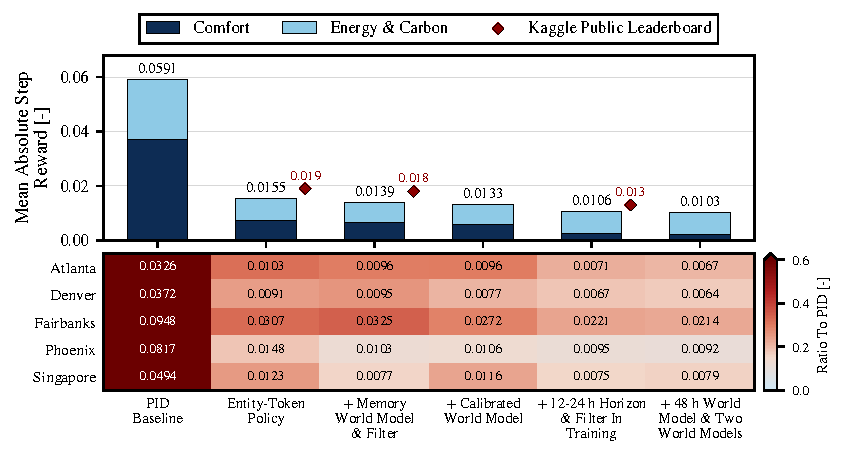
\includegraphics[width=0.94\linewidth]{figures/impact.pdf}
\caption{Score of the PID baseline and of the stages of the method, each adding the change in its label (30 official scenarios, 14 days): reward terms and Kaggle scores (top), climate means colored by ratio to PID (bottom).}
\label{fig:impact}
\end{figure}

\subsection{Where the Gains Come From}
\label{sec:impact}

As can be observed in Figure~\ref{fig:impact}, the first entity-token policy already removes 74\% of the PID score, reducing both terms in every climate. The following stages act on different terms and climates, since the world model with thermal memory and the command filter mainly benefit the warm climates (Singapore and Phoenix), the calibrated world model the cold ones (Fairbanks and Denver) at the expense of Singapore, and the 12 to 24-hour horizon with the filter inside the training rollouts more than halves the comfort term at almost equal energy, thereby improving every climate. Indeed, the filter alone, in rollouts of 6 to 12 hours, worsens the score (0.0182 against 0.0133). The final policy, which adds two alternated world models, the zone memory, a holiday flag and more weekend starts, lowers the comfort term further (to 0.0021) and reaches 0.0103 ($-83\%$), while the six Fairbanks scenarios still account for about 40\% of its loss.

\subsection{Learned Behavior}
\label{sec:behavior}

Figure~\ref{fig:examples} compares the final policy with the PID baseline and the policy with memory and filter in Fairbanks 1 in January (outdoor air below $-35\,^{\circ}$C) and Denver 8 in November.

\begin{figure}[H]
\centering
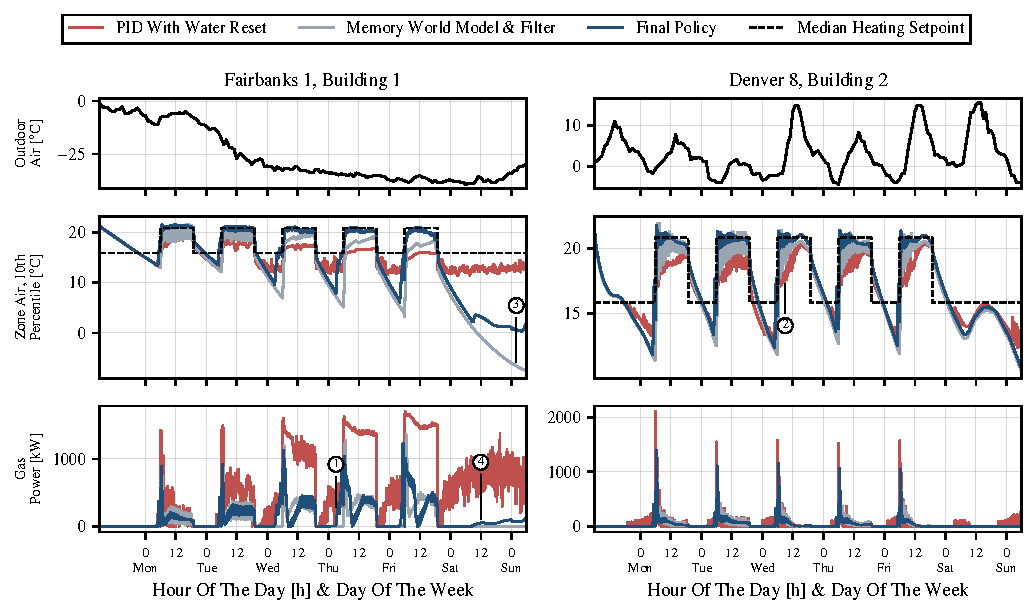
\includegraphics[width=\linewidth]{figures/examples.pdf}
\caption{First week of Fairbanks 1 (from 1 January) and Denver 8 (from 5 November): outdoor air, 10th percentile of the zone temperatures with the median heating setpoint and gas power. The numbered markers are discussed in Section~\ref{sec:behavior}.}
\label{fig:examples}
\end{figure}

As shown, the PID baseline heats all night (marker 1), with 95.8~MWh of gas in the Fairbanks week against 23.9~MWh for the final policy, and still leaves the coldest zones below the setpoint, also in Denver 8 (marker 2). Both learned policies switch the plant off at night and over the weekend, but in Fairbanks 1 the policy with memory and filter lets the coldest zones fall below $-5\,^{\circ}$C (marker 3), whereas the final policy restarts heating on Saturday (marker 4) and keeps the coldest zones at the setpoint until the evening, with 21\% more gas (score 0.0541 against 0.0650), and in Denver 8 it reaches the setpoint sooner (0.0121 against 0.0174).

\subsection{World Models and Training Seeds}
\label{sec:wmseeds}

The three world models of Figure~\ref{fig:analysis} reach similar temperature errors over 24-hour closed-loop rollouts on held-out buildings (0.82, 0.79 and 0.79~K for WM-1, WM-2 and WM-3).

\begin{figure}[H]
\centering
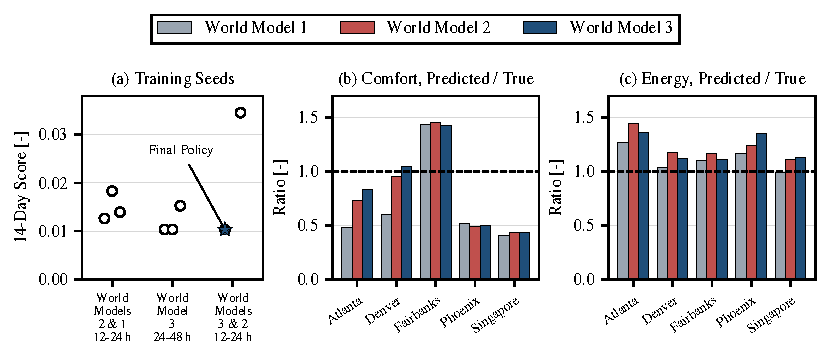
\includegraphics[width=0.84\linewidth]{figures/analysis.pdf}
\caption{(a) 14-day score of every seed of three recipes; (b, c) predicted to true comfort and energy, 24-hour closed loop.}
\label{fig:analysis}
\end{figure}

As can be observed in Figure~\ref{fig:analysis}(a), the training seed weighs as much as the choice of world model, since the recipe of the final policy scores 0.0103 with one seed and 0.0345 with another, and that on WM-3 with a 24 to 48-hour horizon yields 0.0104 in two of three seeds. Figures~\ref{fig:analysis}(b) and (c) show that all three world models underestimate the discomfort by about half in Phoenix and Singapore, overestimate it by more than 40\% in Fairbanks and overestimate the energy, especially in Atlanta and Phoenix, so that their aggregate calibration on comfort (1.00 to 1.08) hides opposite errors that a single comfort factor $\kappa$ cannot compensate. The policy on WM-2 is worse than on WM-1 (0.0121 against 0.0106), yet WM-3, with similar errors, yields the best ones, so that seeds matter more.

\subsection{Remaining Headroom}
\label{sec:headroom}


To bound the gain of better hourly decisions, an oracle clones the simulator every hour, scores 31 modifications of the next-hour commands of the final policy (plant on or off, water, supply-air and reheat offsets) over 24 hours and applies the best, as compared in Figure~\ref{fig:headroom} with world-model scoring.

\begin{figure}[H]
\centering
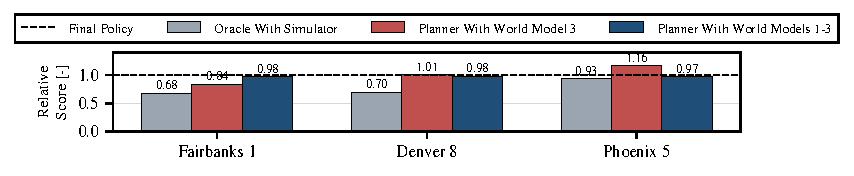
\includegraphics[width=0.8\linewidth]{figures/headroom.pdf}
\caption{Seven-day score of the oracle and of the planners, relative to the final policy.}
\label{fig:headroom}
\end{figure}

 As can be observed, the oracle reduces the score by about 30\% in Fairbanks 1 and Denver 8 and by 7\% in Phoenix 5, while the search scored by WM-3 recovers half of the gap in Fairbanks 1 but worsens Phoenix 5, and the agreement of three world models avoids losses but gains little, at 13 to 33~s per decision, beyond the Kaggle budget.

\section{Conclusion}

This work has shown that a single policy for unseen buildings can be trained through entity-token world-model rollouts, reducing the PID score by 83\%. Since the remaining loss is mostly subarctic and an oracle still recovers about 30\% of it in two scenarios, future work will model the power of each zone coil, to heat only where needed.

\paragraph{Acknowledgments.} To be completed.

\renewcommand{\bibfont}{\footnotesize}
\setlength{\bibsep}{0pt plus 0.5pt}
\bibliographystyle{plainnat}
\bibliography{references}

\end{document}
